\documentclass[12pt,a4paper]{report}

\usepackage{styles/dolgozat}

\usepackage{listings}
\usepackage{styles/cpp}
\usepackage{styles/python}

\usepackage{hyperref}

\begin{document}

\pagestyle{empty}

{\small
Miskolci Egyetem \hfill Miskolci Egyetem

Gépészmérnöki és Informatikai Kar \hfill Gépészmérnöki és Informatikai Kar

Általános Informatikai Intézeti Tanszék \hfill \hfill Alkalmazott Matematikai Intézeti Tanszék}

{\large
\begin{center}
\vglue 1.5truecm

\includegraphics[scale=0.15]{images/me_logo.png}\\
\end{center}}

\vglue 1.5truecm

{\huge
\begin{center}
\textbf{A szakdolgozat címe}
\end{center}}

\vspace*{1cm}

\begin{center}
\LARGE \textbf{Szakdolgozat}
\end{center}

\vspace*{2.5truecm}

{\large
\hspace{6.5cm} \textbf{Készítette}:

%\vskip 2mm

\hspace{6.5cm} \textbf{Név}: Szakdolgozó Neve

%\vskip 1mm

\hspace{6.5cm} \textbf{Neptunkód}: \texttt{NPTNCD}

%\vskip 1mm

\hspace{6.5cm} \textbf{Szak}: Mérnökinformatikus BSc

%\vskip 1mm

\hspace{6.5cm} Korszerű web technológiák szakirány
}

\newpage


\newpage

\pagestyle{empty}

\vspace*{1cm}  
\begin{center}
\large\textsc{\bfseries Eredetiségi Nyilatkozat}
\end{center}
\vspace*{2cm}  

Alulírott \textbf{Megyeri Balázs}; Neptun-kód: \texttt{AXQB0Z} a Miskolci Egyetem Gépészmérnöki és Informatikai Karának végzős Mérnökinformatikus szakos hallgatója ezennel büntetőjogi és fegyelmi felelősségem tudatában nyilatkozom és aláírásommal igazolom, hogy \textit{T5 alapú kérdésgeneráló mintarendszer fejlesztése és hatékonyságelemzése}
című szakdolgozatom saját, önálló munkám; az abban hivatkozott szakirodalom
felhasználása a forráskezelés szabályai szerint történt.\\

Tudomásul veszem, hogy szakdolgozat esetén plágiumnak számít:
\begin{itemize}
\item szószerinti idézet közlése idézőjel és hivatkozás megjelölése nélkül;
\item tartalmi idézet hivatkozás megjelölése nélkül;
\item más publikált gondolatainak saját gondolatként való feltüntetése.
\end{itemize}

Alulírott kijelentem, hogy a plágium fogalmát megismertem, és tudomásul veszem, hogy
plágium esetén szakdolgozatom visszautasításra kerül.

\vspace*{3cm}

\noindent Miskolc, \hbox to 2cm{\dotfill} .év \hbox to 2cm{\dotfill} .hó \hbox to 2cm{\dotfill} .nap

\vspace*{3cm}

\hspace*{8cm}\begin{tabular}{c}
\hbox to 6cm{\dotfill}\\
Hallgató
\end{tabular}

\newpage


\cleardoublepage
\pagenumbering{gobble}
\tableofcontents
\cleardoublepage
\pagenumbering{arabic}

\newpage

\pagestyle{fancy}

\Chapter{Bevezetés}

A természetes nyelvfeldolgozás az informatika egyik legkomplexebb feladatköre. Ennek egyik oka, hogy az emberi nyelv és annak kialakulása szorosan összefügg az emberi aggyal és annak evolúciójával, melyet még a mai napig se sikerült teljesen feltérképeznünk és megértenünk. Nyelvünk értő használata egyike azon utolsó problémaköröknek, amiket a számítógépek eddig nem voltak képesek még megközelítőleg se megfelelően teljesíteni, hiszen akár már egy egyszerű mondat feldolgozásához, kontextusban való elhelyezéséhez vagy akár kibővítéséhez is óriási méretű szabályhalmazokra és számítási teljesítményre van szükség.\\
Vegyük példának ezt a mondatot:

\vspace{0.5cm}
\centerline{,,Ausztriában lopott autóval karambolozott három magyar fiatal.''}
\vspace{0.5cm}

\noindent Ez a mondat akár 4 különböző jelentést is takarhat:

\begin{itemize}
\item Az autót Ausztriában tulajdonították el és így karamboloztak.
\item Ausztria területén történt a karambol.
\item Az autó amiben ültek lopott volt.
\item Az autó amivel összeütköztek volt lopott.
\end{itemize}

Mind a 4 értelmezés helyes nyelvtanilag és értelmezésük pusztán attól függ, hogy hogyan tagoljuk a mondatot az elemzés során. Természetesen a mondat pontos jelentése egyértelművé válik, amint megismerjük a kontextust, amelyben a mondat elhangzott, de mindehhez komplex háttértudásra van szükségünk. Ennek a háttértudásnak az ismerete hiányzott eddig a különböző NLP feladatok megoldására írt programokból, hiszen ezek rengeteg adatot, metaadatot, szabályt és egyéb heurisztikát igényelnek. Mi emberek az evolúció, illetve az egyéni fejlődés során gyerekkortól megismertük ezt a szükséges háttértudást egy ilyen mondat értelmezéséhez, viszont a gépek nem rendelkeztek eddig az ehhez szükséges eszköztárral. 


\Chapter{Természetes nyelvfeldolgozás}

\Section{A fejezet célja}

Ez a fejezet még nem a saját eredményekkel foglalkozik, hanem bemutatja, mi a problémakör, milyen módszerekkel, milyen eredményeket sikerült elérni eddig másoknak.

A hivatkozások jelentős része ehhez a fejezethez szokott kötődni.
(Egy hivatkozás például így néz ki \cite{coombs1987markup}.)
Ez szintén egy példa internetes hivatkozásra, a CSS szabvány kapcsán \cite{css}.
Itt lehet bemutatni a hasonló alkalmazásokat.

\Section{Tartalom és felépítés}

A fejezet tartalma témától függően változhat. Az alábbiakat attól függően különböző arányban tartalmazhatják.
\begin{itemize}
\item Irodalomkutatás. Amennyiben a dolgozat egy módszer kidolgozására, kifejlesztésére irányul, akkor itt lehet részletesen végignézni (módszertani vagy időrendi bontásban), hogy az eddigiekben milyen eredmények születtek a témakörben.
\item Technológia. Mivel jellemzően kutatásról vagy szoftverfejlesztésről van szó, ezért annak a jellemző elemeit, technikai részleteit itt kell bemutatni.
Ez tehát egy módszeres bevezetés ahhoz, hogy ha valaki nem jártas a témakörben, akkor tudja, hogy a dolgozat milyen aktuálisan elérhető eredményeket, eszközöket használt fel.
\item Piackutatás. Bizonyos témáknál új termék vagy szolgáltatás kifejlesztése a cél.
Ekkor érdemes annak alaposan utánanézni, hogy aktuálisan milyen eszközök érhetők el a piacon.
Ez szoftverek esetében a hasonló alkalmazások bemutatását, táblázatos formában történő összehasonlítását jelentheti.
Szerepelhetnek képek és észrevételek a viszonyításként bemutatott alkalmazásokhoz.
\item Követelmény specifikáció. Külön szakaszban érdemes részletesen kitérni az elkészítendő alkalmazással kapcsolatos követelményekre.
Ehhez tartozhatnak forgatókönyvek (\textit{scenario}-k).
A szemléletesség kedvéért lehet hozzájuk képernyőkép vázlatokat is készíteni, vagy a használati eseteket más módon szemléltetni.
\end{itemize}

\Section{Amit csak említés szintjén érdemes szerepeltetni}

Az olvasóról annyit feltételezhetünk, hogy programozásban valamilyen szinten járatos, és a matematikai alapfogalmakkal sem ebben a dolgozatban kell megismertetni.
A speciális eszközök, programozási nyelvek, matematikai módszerekk és jelölések persze jó, hogy ha említésre kerülnek, de nem kell nagyon belemenni a közismertnek tekinthető dolgokba.

\Chapter{Neurális hálózatok a nyelvfeldolgozásban}

Az első jelentős fejlődés a területen a neurális hálózatok megjelenése volt. Korábban számos próbálkozás született szabályok, sablonok, statisztikai megoldások felhasználásával, azonban ezek például egy chatbot vagy szöveggenerálási feladat esetén hamar problémákba ütköztek, hiszen egy újabb, addig ismeretlen nyelvi elem vagy egy speciálisabb kontextus teljesen meg tudta állítani ezen programok működését. További probléma volt, hogy mivel magát a nyelvet, annak kódolását és dekódolását is emberek találták ki emberi aggyal, így egyszerű képletekkel, szabálybázisokkal ez a probléma nem volt megoldható, mivel az emberi agy - mint az számos kutatásból kiderült - nem használja beépítve ezeket a működéseket, például nem kezdi el egyenként, szekvenciálisan feldolgozni a betűket, hanem belső állapotától függően képes egyben látni szavakat, mondatokat és leginkább predikciókkal dolgozik, mint sem pontosan leírt, kötött műveletekkel, szabályokkal.

Mindezen problémák miatt logikus lépés volt megvizsgálni az emberi agyat és előállni egy olyan koncepcióval, mely képes modellezni az agy mintafelismerési képességét és ezáltal új távlatokat nyitni a nyelvfeldolgozás területén. Ezek voltak a \textbf{neurális hálózatok}.

Az idők során számos neurális hálózat típus jelent meg: perceptron, feed forward, MLP, konvolúciós, visszacsatolt(RNN) stb. Ezek közül számunkra a nyelvfeldolgozás területén a legfontosabb és legtöbbet használt típus az RNN(Recurrent Neural Network).

A neurális hálózatok felépítése nagyon változatos lehet, azonban számos közös jellemzőjük akad. Minden hálózatnak tartalmaznia kell egy bemeneti réteget, egy rejtett réteget és egy kimeneti réteget. Ezen rétegek jellege a feladat típusától függően változtatható, például a hálózat bemenete lehet többdimenziós, a rejtett rétegekben változtathatjuk a neuronok kötéseit, illetve az adatmozgások irányát, a kimenete pedig lehet egy skalár mennyiség vagy egy vektor, attól függően, hogy osztályozni vagy regressziót számítani szeretnénk.

\textbf{RNN} esetén a feladat egy szekvencia feldolgozása, ami lehet egy kép, amit szeretnénk felcímkézni, hangfájlok, amik segítségével beszédet szeretnénk felismerni, illetve akár egy szöveg, amit szeretnénk lefordítani vagy értelmezni. Ami közös ezekben a feladatokban, hogy mindegyik problémakör esetén a feldolgozás során a hálózat bemenete és kimenete jelentősen függ egymástól, vagyis a szekvencia egyes elemeinek értelmezése függ a korábbi elemek értelmezésétől.

\begin{figure}[h]
\centering
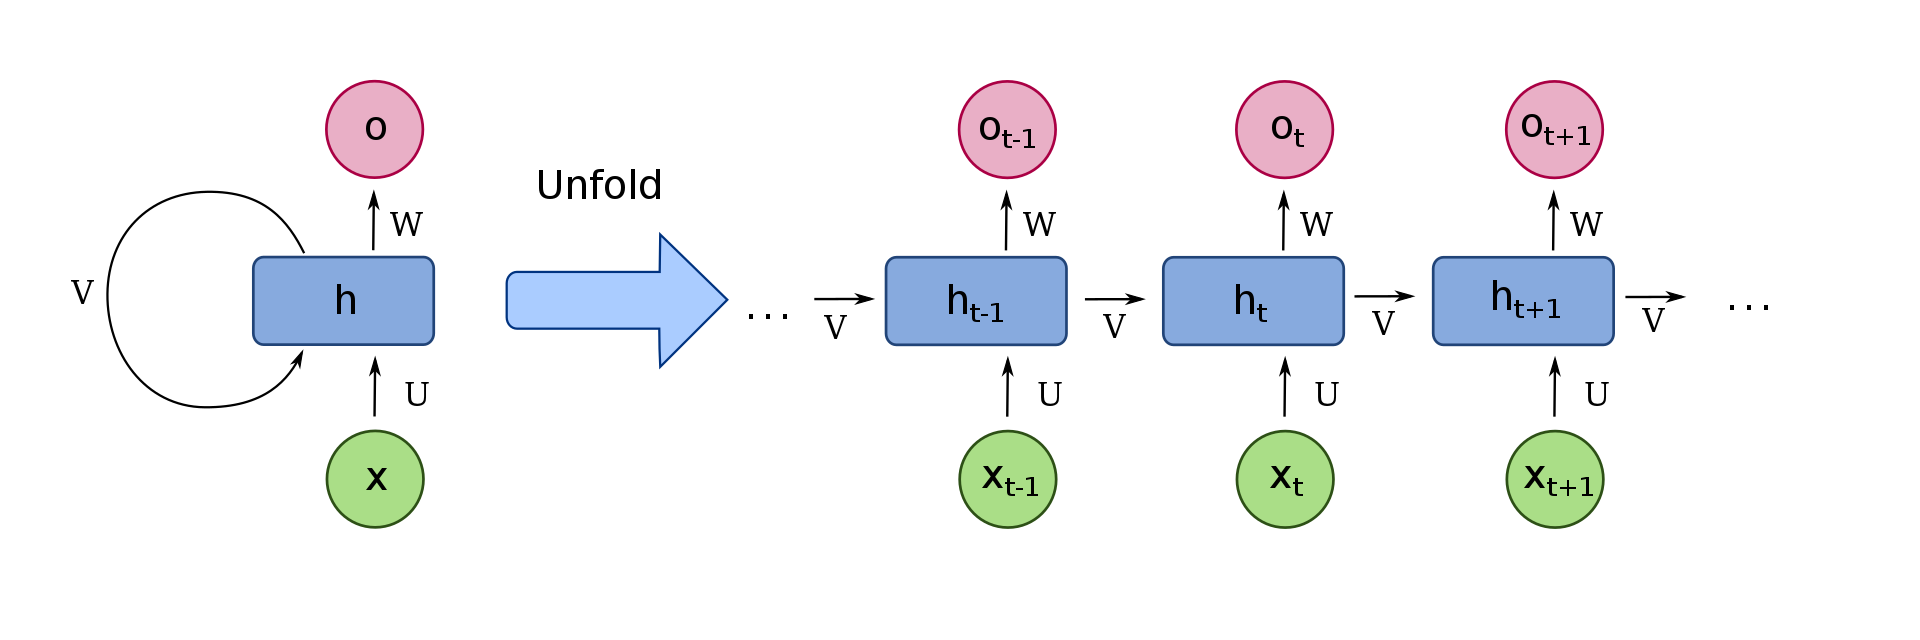
\includegraphics[scale=0.2]{images/rnn.png}
\caption{Az RNN működése \cite{rnn}.}
\label{fig:rnn}
\end{figure}

Kiváló példa erre a szövegfordítás, hiszen a fordítás során fontos a szavak rendje, tehát a hálózatnak sorban, egymás után kell vennie a forrásszöveg szavait és kimenetén ezen szavak adott nyelvű megfelelőjének kell megjelennie.

Ez a működés jelentős előrelépés volt, azonban számos probléma felmerült ennek kapcsán. Az egyik ilyen probléma a hosszabb szövegek értelmezése volt. Ilyenkor a hálózat egyszerűen elfelejtette azt a tudást, amit a szöveg értelmezésének elején megszerzett, ezt hívjuk “vanishing gradients” problémának. Ennek magyarázata a hibafüggvény gradiensében keresendő, ami nem más, mint a hibafüggvény deriváltja a hibagörbe mentén. Amikor ez a gradiens túl kicsi, akkor idővel még kisebbé válik és ezekkel az alacsony, nagyon 0-hoz közeli értékkellel kezdi el frissíteni a hálózat súlyait, egészen addig, amíg azok le nem nullázódnak. Ebben az esetben a hálózat nem tanul tovább. Ennek a problémának létezik a fordítottja is, az “exploding gradients”, melynek során a gradiens túl nagy lesz, ezáltal egy instabil modellt alkotva, melynek hatására a súlyok túl nagyok és idővel NaN értékűek lesznek.

Ezen problémákra születtek megoldások, például a hálózat komplexitásának csökkentése, vagyis a rejtett rétegek számának redukálása, azonban ez nem mindig vezet optimális megoldásra.

Egy másik probléma az RNN-el, hogy a hálózat szekvenciális feldolgozásra készült mivoltából adódóan egyszerűen nem jól párhuzamosítható, vagyis a mai modern hardverekkel, például egy rengeteg, erőteljes párhuzamosításra használható maggal felszerelt GPU-n nem tudjuk effektíven tanítani a hálózatot, ami a nagyobb szövegek értelmezését rettentően időigényessé teszi.

Az RNN tehát minden problémájának ellenére is hatalmas sikereket ért el az NLP területén, azonban 2017-ben egy új neurális hálózat típus jelent meg:\\
az átalakító(transformer), ami a fentebb említett problémákat javítva és a fejlesztést is egyszerűbbé téve átvette a vezetést a szövegfeldolgozás területén.

Az átalakítókat a Google és a Torontói Egyetem szakemberei fejlesztették ki 2017-ben és meg is jelentettek egy cikket "Attention Is All You Need"\cite{attention} címmel, amiben részletezték ezen átalakítók működését. Talán a legnagyobb újítás a párhuzamosíthatóság területén jelent meg, mivel ezeket a hálózatokat a megfelelő eszközökkel hatalmas mennyiségű adatokkal lehet tanítani. Például a Google T5 nevű átalakító modelljének a többnyelvű változatát a c4/multilingual nevű adathalmazzal tanították, ami 26.76 TiB méretű(1 TiB = 1.1 TB). Később az OpenAI vállalat GPT-3 nevű modellje még ezt is túlszárnyalta szinte a teljes publikus internetet tartalmazó 45 TB méretű szöveges adatot tartalmazó tanítóadatával. Ezen méretű tanítóhalmaz korábban elképzelhetetlen volt az RNN-ek használatával.\\
Az átalakítók működését 3 fontos fejlesztésre lehet lebontani:

\begin{itemize}
\item Pozíciókódolások(Positional Encodings)
\item Figyelem(Attention)
\item Önfigyelem(Self-Attention)
\end{itemize}

A \textbf{pozíciókódolással} a korábbi RNN-ek szekvencialitását oldották fel azáltal, hogy a mondatokat nem a szavak sorrendjében kezdték el feldolgozni, hanem a mondat minden szavát ellátták egy annak mondatban elfoglalt pozícióját jelentő címkével. Ez a struktúra szó-sorszám párokat jelent, amiket a hálózat megtanul hatásosan használni. Ennek segítségével a szavak sorrendje immáron nem a hálózat struktúráját jelenti, vagyis a szekvencialitást, hanem egyszerű feature-nek, adatnak tekinthető.

A \textbf{figyelem} egy olyan mechanizmus, melynek segítségével a modell végigmehet a bemenet minden szaván és megadhatja egy szónak a jelentését az alapján, hogy melyik ismert idegennyelvű szóhóz áll a legközelebb a szintaktikája. Ezt a tudást a tanítás során szerzi meg a modell, ezért is van szükség minnél nagyobb adathalmazokra. Ez a működés elsősorban a modell célterületén vagyis  szövegfordítások esetén hasznos, ahol egy adott nyelvű mondat fordításánál a szórend változhat, és nem elég szimplán az egyes szavakat lefordítani, hanem szükség van egyfajta háttértudásra, nyelvi ismeretekre a fordítás során. Pélául a \textit{"The agreement on the European Economic Area was signed in August 1992."} angol nyelvű mondat francia fordítása \textit{"L'accord sur la zone économique européenne a été signé en août 1992."} Láthatjuk, hogy a \textit{"European Economic Area"} fordítása \textit{"la zone économique européenne"}, tehát a szórend és a szavak alakja is változik. Ebben az esetben nem elég az egyes szavakat szekvenciálisan fordítani, hanem minden angol szóhoz a forrásmondatban fel kell építeni egyfajta hőtérképet a francia fordításokkal és a modellnek végig kell néznie az egyes szavakat és meg kell mondania, hogy melyik angol szóhoz melyik francia szó illeszkedik. Esetünkben például az \textit{"European"} szóhoz illeszkedik az \textit{"européenne"} és az \textit{"économique"} szó is, azonban a modell korábbi tanításából adódóan tudja, hogy itt az \textit{"européenne"} fordítás lesz a helyes.

\begin{figure}[h]
\centering
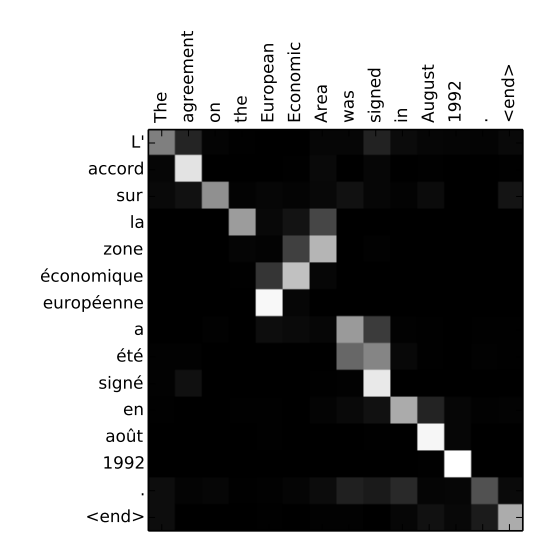
\includegraphics[scale=0.9]{images/translate_heatmap.png}
\caption{Angol-francia fordítás hőtérképe \cite{translation}.}
\label{fig:translate_heatmap}
\end{figure}

Az utolsó fontosabb fejlesztés az \textbf{önfigyelem}, ami talán a legfontosabb a szövegértelmezés szempontjából. Korábban láthattuk, hogy a figyelem segítségével a modell képes megfelelő sorrenben fordítani a szavakat, azonban ez még nem elég ahhoz, hogy képes legyen érteni is az egyes szavak jelentését és ezáltal más szövegfeldolgozási feladatokat is meg tudjon oldani. Ennek érdekében szükségessé vált, hogy a modell mögött álló neurális hálózat felépítsen egy belső reprezentációt az adott nyelvről. Ez a belső működés leginkább a különböző képfelismerési hálózatok(CNN) rétegeihez hasonló, ahol az egyes régetek képesek felismerni éleket, alakzatok és egyéb magasabb szintű, komplexebb struktúrákat, mint emberek, állatok vagy tárgyak. Nyelvi környezetben ezen rétegek képesek felismerni a különböző nyelvtani szabályokat, szinonímákat és szövegrészleteket. A célja ezen rétegeknek, hogy minnél jobban megtanulják az egyes nyelvtani elemeket és kontextusokat, így a modell képes lesz szinte bármilyen nyelvi feladatot megoldani.\\
Vegyük példának a következő angol nyelvű mondatokat:

\begin{enumerate}
\item \textit{"Server, can I have the check?"}
\item \textit{"Looks like I just crashed the server."}
\end{enumerate}

A \textit{"server"} szó ebben a 2 mondatban 2 különböző jelentéssel bír: az egyik mint felszolgáló vagy pincér, míg a másik egy webes kiszolgálóra utal. Mi emberek a \textit{"server"} szó körül lévő szavakból könnyen meg tudjuk különböztetni a 2 jelentést, azonban ez a gépeknek korábban nem volt egyszerű feladat. Az önfigyelem erre a feladatra nyújt megoldást azáltal, hogy képes az egyes szavakat más szavakhoz kötni és így a modell megtanulja, hogy abban az adott kontextusban mit is jelenthet az a szó. Például az 1. mondatban a \textit{"server"} szó mellett megtalálható a \textit{"check"}, a \textit{"can"} és a \textit{"have"} szó is, melyek együtt sűrűbben szerepelnek egy éttermi szituációt leíró kontextusban, mint a webfejlesztés esetében, tehát itt egy pincért jelent a szó, míg a 2. mondatban megtalálható a \textit{"crashed"} szó, ami pedig az informatikában és webes környezetekben gyakoribb, ezáltal a \textit{"server"} itt egy webkiszolgálót jelent.

\begin{figure}[h]
\centering
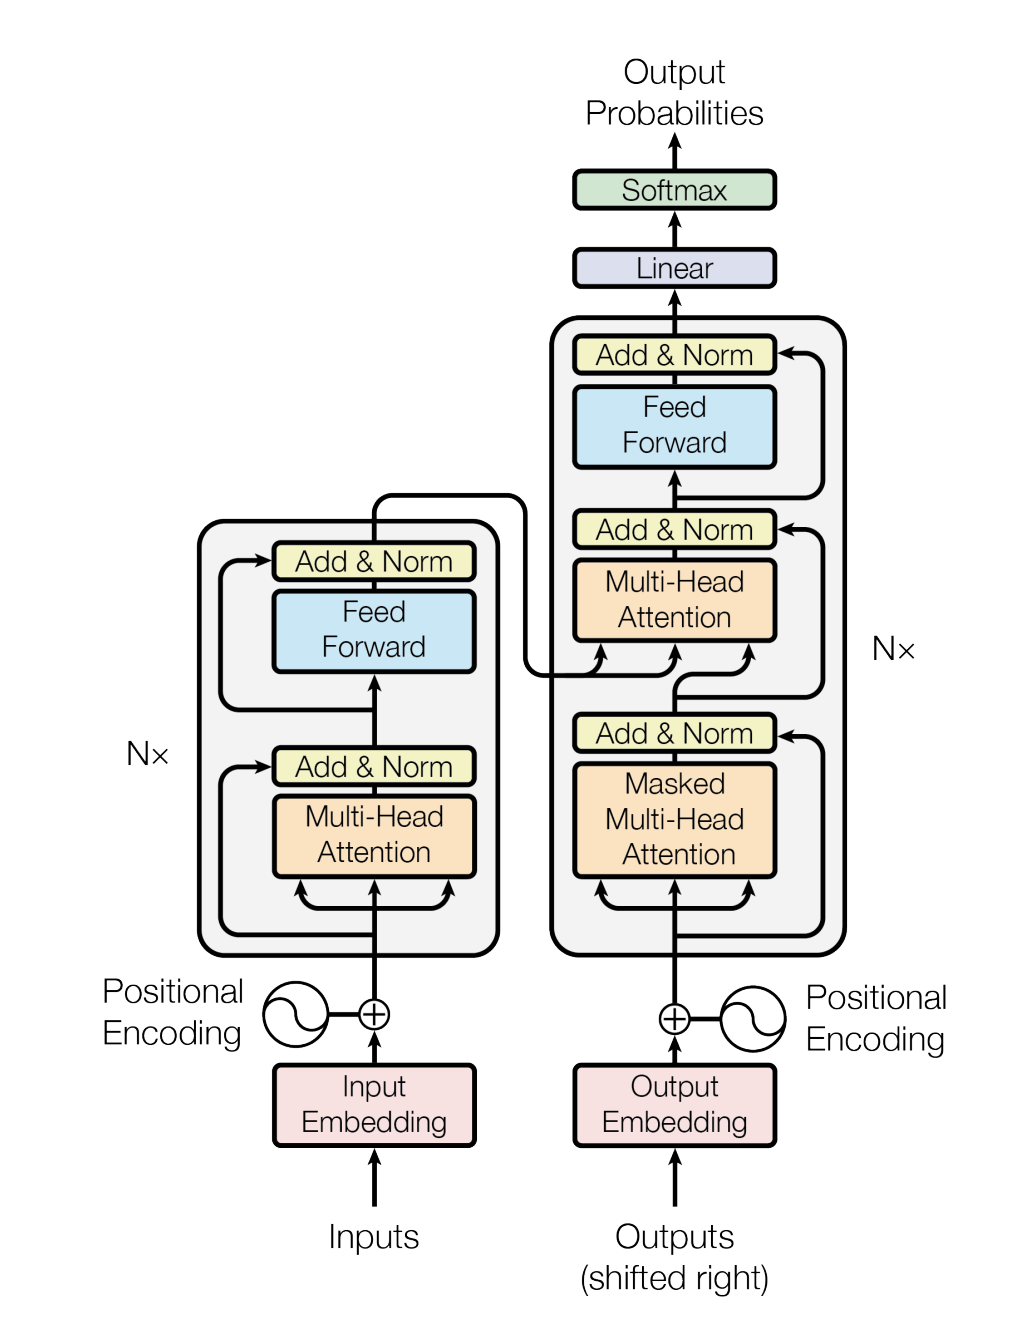
\includegraphics[scale=0.4]{images/transformer.png}
\caption{Az átalakító modell architektúrája  \cite{attention}.}
\label{fig:transformer}
\end{figure}

Ez a 3 fontosabb fejlesztés indítottal el útjára az átalakító alapú modelleket, melyek közül az első jelentősebb a Google által 2018-ban kifejlesztett \textbf{Bidirectional Encoder Representations from Transformers(BERT)} volt. A BERT nem csak egy újfajta modell architektúra volt, hanem egy teljesen új betanított modell, amit ingyenesen letölthetővé is tettek. Kisebb átalakításokkal számos probléma megoldására képes volt: szövegösszefoglalás, kérdés-válasz generálás, osztályozás és még sok más feladat. Működésének legfontosabb fejlesztése az átalakító modell kétirányú kiterjesztése volt. Korábban az átalakító modellek a tanítás során balról jobbra vagy kombináltan balról jobbra és jobbról balra dolgozták fel a szövegeket. Ezzel szemben a BERT a szavak értelmezésénél a környező szavakat mind a két lehetséges irányban egyszerre dolgozza fel, ami a szövegek mélyebb megértését teszi lehetővé.\\
Ahhoz, hogy ez a működés megvalósuljon 2 fajta tanítási stratégiát használ a BERT:

\begin{itemize}
\item Masked-Language Modeling (MLM)
\item Next Sentence Prediction (NSP)
\end{itemize}

A \textbf{Masked-Language Modeling} az adott szöveg, pontosabban a szöveg szavainak mélyebb megértését célozza. A BERT hálózat tanítása során az egyes mondatok szavainak kb. 15\%-át kicserélik [MASK] tokenekre. Ezt követően a modell megpróbálja kitalálni ezeket a maszkolt szavakat a körülötte lévő nem maszkolt szavak kontextusa alapján. A predikció során a maszkolt szavak mindkét oldaláról figyelembe veszi a nem maszkolt szavak kontextusát, innen ered a kétirányúsága a modellnek. Ez a működés nagyon hasonlít ahhoz, ahogy mi emberek értelmezünk egy szöveget vagy próbáljuk kitalálni egy ilyen feladat során a hiányzó szavakat.

\begin{figure}[h]
\centering
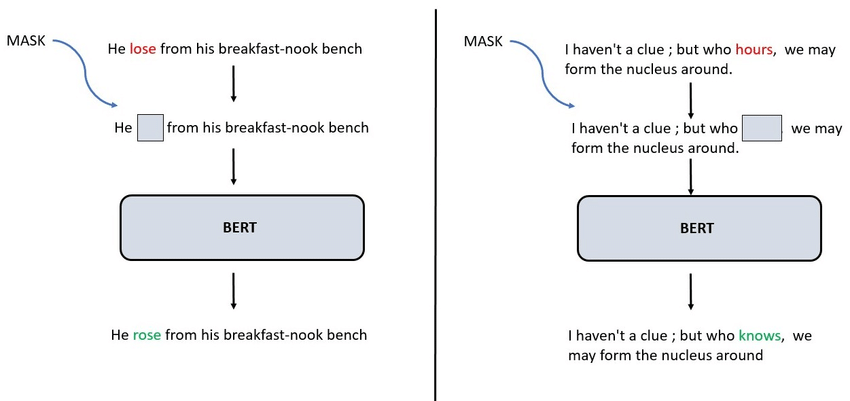
\includegraphics[scale=0.4]{images/bert_mask.png}
\caption{Maszkolt szavak beillesztése a BERT működése során \cite{bert}.}
\label{fig:bert}
\end{figure}

A \textbf{Next Sentence Prediction} esetén az MLM-el szemben nem a szöveg szavainak a megértése a cél, hanem az egyes mondatok közötti kapcsolatok feltárása. Ennek érdekében a tanítás során a modell mondat párokat kap, melyek második eleméről el kell döntenie, hogy az első mondat után következnek-e az eredeti forrásszövegben. A gyakorlatban a bemeneti szöveg mondatainak 50\%-a olyan páros, ahol a mondatok egymás után következnek, a másik 50\%-a pedig olyan, ahol a második mondat random kerül kiválasztásra és feltesszük, hogy a random mondat nem lesz kapcsolatban az első mondattal.

\begin{figure}[h]
\centering
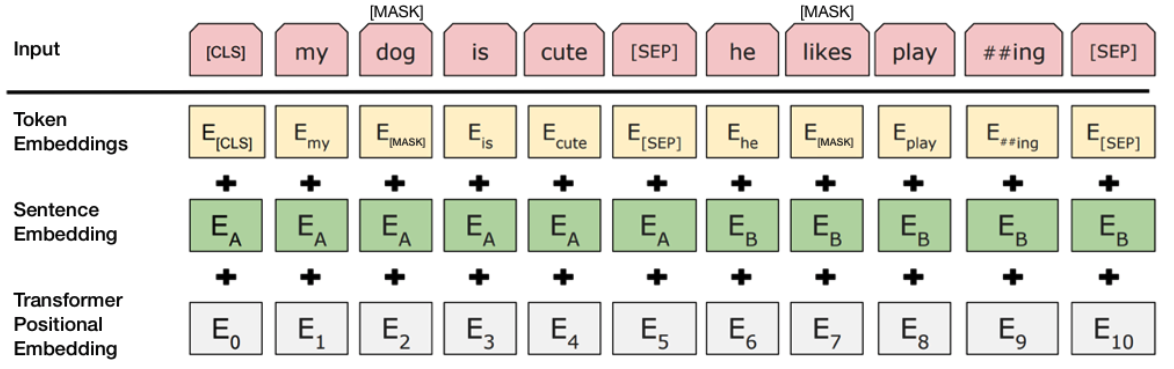
\includegraphics[scale=0.3]{images/next_sentence_prediction.png}
\caption{Next Sentence Prediction a gyakorlatban \cite{bert2}.}
\label{fig:bert2}
\end{figure}

A BERT jelentős sikerei után elkezdődtek a kutatások a modell felhasználók számára való egyszerűsítésére, adathalmazának kibővítésére és tisztítására, illetve a modell képességeinek újabb feladatokra történő kiterjesztésére. 2020-ban a Google kutatói elő is álltak a \textbf{T5} nevezetű modellel. A modell fő célja az volt, hogy a korábbi fejlesztésekkel ellentétben a modell bemeneti forrásszövege és a kimenet is egységes szöveg formátumú legyen minden NLP feladat esetén.

A modell előtanítása során a Colossal \textbf{Clean Crawled Corpus(C4)} nevű adathalmazt használták, ami közel 700 GB méretű és a  Common Crawl adathalmaz egy tisztított verziója. A C4 adathalmaznak létezik többnyelvű változata is az \textbf{mC4}, amely már tartalmazza a magyar nyelvet is sok más nyelv mellett. Az mC4 adathalmazon tanított T5 pedig az \textbf{mT5} nevet viseli és képes magyar nyelvű szövegek generálására is.

Belső működésében a T5 hasonlóan működik mint a BERT. A Masked-Language Modeling ugyanúgy megmaradt, azonban kibővítették azzal, hogy immáron nem csak egy-egy szót, hanem egyszerre több egymás melletti szót is maszkol, amit a modellnek ugyanúgy ki kell majd találnia. Ennek érdekében a forrásszöveget bemenet-cél párosokra bontja és ezeket fogja megtanulni a tanítás során. A BERT-el ellentétben itt a kimenet nem egyetlen szó lesz, hanem egy generált szöveg, tetszőleges mérettel.

\newpage

\begin{figure}[h]
\centering
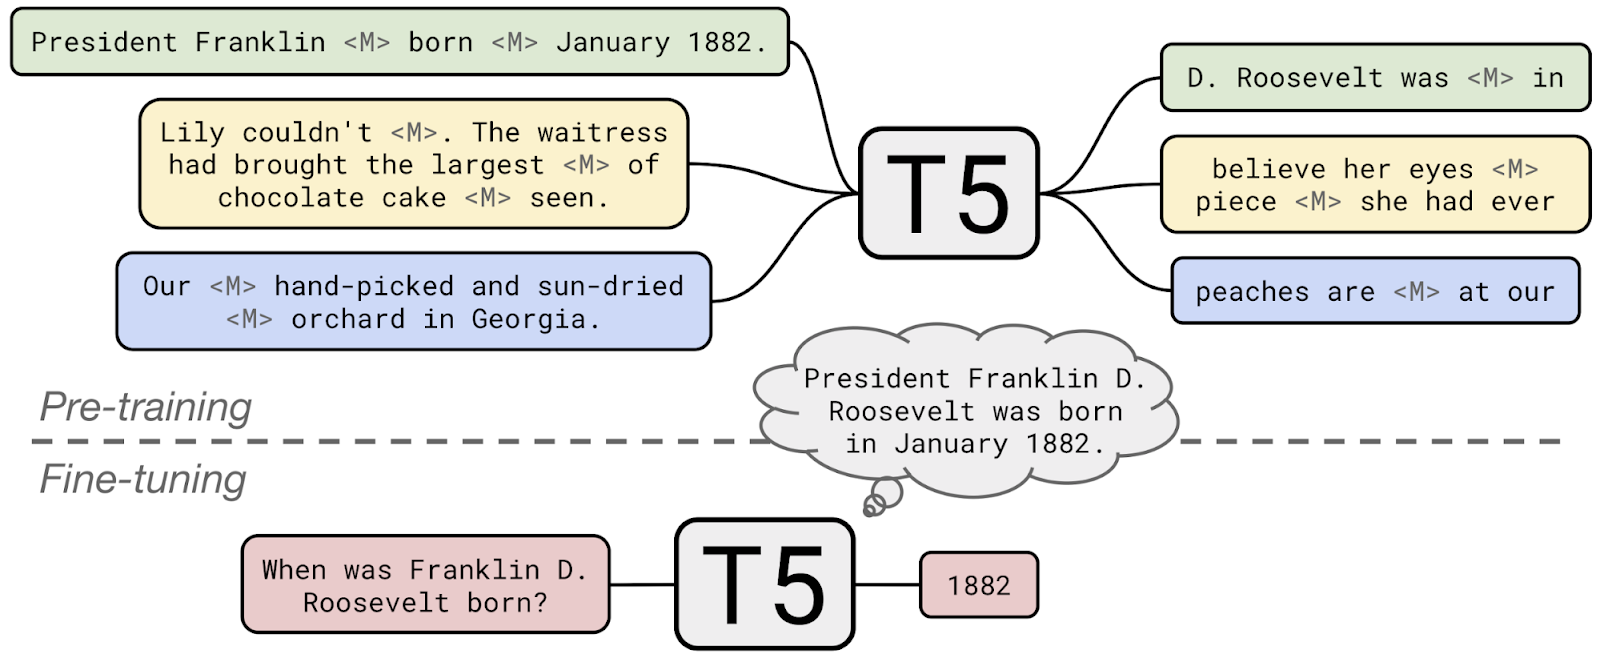
\includegraphics[scale=0.2]{images/t5.png}
\caption{T5 modell a tanítás előtt és után \cite{t5}.}
\label{fig:t5}
\end{figure}

Az előtanítás után a modellt finomhangolták számos NLP feladatra: fordítás,\\
összegzés, mondathasonlóság stb. A finomhangolás során bevezettek egy egyedi formátumot a különböző feladatok különválasztására. A forrásszöveg elé beszúrtak egy prefixet, ami az adott NLP feladatot jelöli. Ennek formátuma:

\textbf{feladat\_ azonosítója: forrászöveg}

Ez azért volt szükséges, hogy a modell súlyait feladatok szerint tudják csoportosítani és így az egyes feladatokra való finomhangolás nem zavar bele a többi feladat megoldásába.
\Chapter{A kérdésgeneráló webalkalmazás megvalósítása}

Ezen fejezet célja az általam készített kérdésgeneráló mintaalkalmazás bemutatása. Terítékre kerül az alkalmazás célkitűzése, tervezése, fejlesztési menete, végül pedig az alkalmazás tesztelése, mind automatikus, mind pedig manuális formában. Kitérek továbbá a felhasznált programozási eszköztárak bemutatására, azok előnyeivel és hátrányaival együtt.

\Section{Az alkalmazás célja}

Ez a webalkalmazás a dolgozatomban bemutatott módszerek gyakorlati alkalmazásának bemutatására szolgál. Az alkalmazás alapvetően egy online kérdésgenerátor, melynek meg lehet adni egy szöveges kontextust és az alapján a program mögött álló modell generál bizonyos számú kérdést. A célom az volt, hogy biztosítsak egy nagyon egyszerű, átlátható és jól kezelhető interfészt, továbbá hogy maga az algoritmus is minél relevánsabb kérdéseket alkosson meg. Mindezt online formában képzeltem el, hiszen az alkalmazás szerver oldali(backend) része meglehetősen erőforrás-igényes, így azt egy egyszerű asztali alkalmazás formájában nehéz lenne futtatni, illetve így bárhonnan szabadon elérhetővé válik a program.

\Section{A programmal szemben támasztott \\ követelmények}

\begin{itemize}
\item \textbf{Gyors válaszidő, optimális működés}: Mivel az alkalmazás mögött egy nagyobb neurális hálózat van, így mindenképp biztosítani kell, hogy a szerver rendelkezzen a megfelelő mennyiségű memóriával, processzormaggal vagy akár videokártyával, annak érdekében, hogy reális válaszidőket kapjon a felhasználó. Továbbá a kódnak is alkalmazkodnia kell a körülményekhez, így rövidnek, átláthatónak és gyorsnak kell lennie.
\item \textbf{Letisztult felhasználói interfész}: Az alkalmazás alapvető céljából fakadóan biztosítani kell az egyszerű kezelhetőséget. Alkalmasnak kell lennie tetszőleges méretű szöveges kontextus feldolgozására, illetve a generált kérdéseknél is törekedni kell a könnyű másolhatóságra, hogy a felhasználó később be tudja illeszteni dokumentumaiba őket.
\item \textbf{Megfelelő minőségű kérdések}: Az alkalmazás által kreált kérdések nem térhetnek el a megadott kontextustól, de törekedni kell arra, hogy ne csak a megadott szövegből kimásolva kérdezzen, hanem érződjön valamilyen háttértudás is a kérdések mögött. Illetve a kérdéseknek az adott nyelven értelmesnek kell lenniük.
\item \textbf{Általános tudásbázis}: Szükség van arra, hogy az alkalmazás minél több témakörből képes legyen kérdéseket generálni, így olyan tanítóhalmazra van szükség, ami nem korlátozódik egyetlen témára, illetve több kérdés típust is tartalmaz.
\end{itemize}

\Section{A program megtervezése}

Az alkalmazás elkészítését hosszas tervezőfolyamat előzte meg. Első lépésként választani kellett egy megközelítési módot az alapfeladat megvalósításához. Számos módszertan létezik a kérdésgeneráláshoz, de én végül a neurális hálózat alapú megoldás mellett döntöttem, azon belül is a már részben előtanított transformer modellek mellett, melyek már rendelkeznek alapvető háttértudással, így már csak a kérdésgenerálás megvalósítására kell megtanítani őket.

Következő lépésként el kellett dönteni, hogy milyen nyelven történjen a kérdésgenerálás. Itt szükséges volt összeszedni, hogy az egyes nyelveken milyen mennyiségben áll rendelkezésre tanítóhalmaz a neurális hálózat tanításához, hiszen elengedhetetlen, hogy a hálózat lásson kontextusokat és hozzájuk készült kérdéseket mintának, ami alapján később képes lesz saját magától is hasonló kérdéseket alkotnia. Végül az angol nyelvre esett a választás, mert ezen a nyelven találtunk megfelelő tanítóhalmazt és a feladathoz illő alaptudással rendelkező hálózatot, melyet később tovább tudtunk tanítani.

Ezután a megfelelő transformer hálózat kiválasztása következett. Számos hálózat létezik, melyekkel megoldható a feladat, azonban a legtöbbjük vagy már elavult, vagy fizetős az elérése, így végül a modernebb és nagyobb tudású, ingyenesen elérhető T5 nevű modell mellett döntöttem.

Mivel az alkalmazás céljai között szerepel, hogy online elérhető legyen, így ezután elkezdődhetett a szerveroldali működés kidolgozása. A szerver programozási nyelvénél a Python-ra esett a választás, mivel nagyon hasznos könyvtárai vannak adatelemzés és statisztika területén, illetve webfejlesztési területen elérhető hozzá egy Django nevű szerveroldali keretrendszer is, mely jelentősen megkönnyítette a szerver elkészítését. Magának a szervernek egyetlen főbb végpontot kellet biztosítani, ami a megadott szöveges kontextust fogadja és válaszként visszaadja az elkészült kérdéseket. Miután az alkalmazás nem tárol felhasználói adatokat, így adatbázisszerver nem lett konfigurálva hozzá, de a rendszer úgy lett kialakítva, hogy ha idővel mégis szükség lenne rá, akkor könnyen be lehet csatlakoztatni egy tetszőleges adatbázist. 

Mindezek mellett szükségessé vált időközben, hogy magának a neurális hálózatnak a tanítását és működését valamilyen szinten szeparáljuk a szervertől, hiszen ez a feladatrész akár napokig is eltarthat még erősebb hardver esetén is. Ezért született az a döntés, hogy a tanításért felelős kódokat vegyük külön egy önmagában futtatható kódfájlba, melyet bárhol képesek vagyunk futtatni, például valamilyen felhőszolgáltatáson és utána a betanított hálózatot, ha van rá lehetőség mentsük el egy tárhelyre, majd onnan a szerver töltse be és már készen, előtanítva használja azt. A tanításért felelős felhőszolgáltatásnak a Google Colab nevű rendszerét használtuk, míg a betanított hálózatot a Hugging Face nevű oldalon tároltuk el, ahonnan egy egyszerű API-n keresztül könnyen le is tudtuk tölteni saját szerverünkre, ahol egyszerű fájlként tud tárolódni.

Miután megterveztük a szervert következhetett a kliensoldali(frontend) rész. Itt a Vue.js nevű frontend keretrendszert választottuk, mivel kisméretű, gyors és könnyű benne a fejlesztés is. A rendszer komponensalapú megközelítése segítette az alkalmazás egyszerű és átlátható működésének biztosítását. Az klienshez igyekeztünk letisztult dizájnt választani, melyen egyértelmű minden funkció és biztosított, hogy a felhasználó a program minden funkciójának tudja a szerepét. Szempont volt például, hogy tetszőleges méretű kontextust tudjon kezelni a kliens, illetve, hogy a kérdések együtt és külön-külön is kimásolhatóak legyenek a későbbi felhasználásukhoz. A felületen történő navigációt pedig ikonok és apró súgószövegek segítik.

Az utolsó lépés a tesztek és tesztesetek előkészítése volt. A jelenlegi és jövőbeli fejlesztés megkönnyítése érdekében szükséges volt automatizált teszteket készíteni, mint például egységteszteket és integrációs teszteket. Mindezeket kliens és szerveroldalon is el kellett készíteni. Továbbá, mivel egy NLP feladatot oldunk meg, így szükségessé vált a manuális, kézi tesztelés is különböző tesztesetekkel. Elsőkörben természetesen az alap eseteket kellett vizsgálni, hogy egyáltalán értelmes kérdések készülnek-e, majd pedig következhettek a komplexebb szituációkat bemutató tesztek.

\Section{Telepítés és futtatás}

Mivel alkalmazásunk alapvetően webes környezetbe lett szánva, így lokális futtatása nem feltétlenül egyszerű feladat, de azért törekedtünk a könnyű elindítás biztosítására. Ennek érdekében elérhetővé tettük az alkalmazást Docker környezetben. A Docker használatához mindössze a Docker Desktop nevű alkalmazás telepítése szükséges, amely elérhető Windows, Linux és MacOS operációs rendszereken is. Ekkor a frontend és backend rész együttes futtatása mellet a http://localhost:3000 cím alatt válik elérhetővé az alkalmazás.

Azonban a tesztelés megkönnyítése végett éles környezetben is elérhetővé tettük a webalkalmazást a következő URL alatt:

\vspace{1cm}

\centerline{\url{https://mb-thesis-t5-qg-frontend-oumla56ewq-lm.a.run.app}}

\vspace{1cm}

Az éles környezetet a Google Cloud biztosítja számunkra, ahol bizonyos mennyiségű havi szerver felé indított kérésig ingyenesen biztosítanak nekünk lehetőséget alkalmazásunk tárolására. A nap első indításánál lassabb lehet az oldal betöltése, de általában gyorsan el lehet érni a weboldalt és a kérdésgenerálás se tart túl sokáig a biztosított hardvereken.

Az alkalmazás lokális elindításához elengedhetetlen néhány alapkövetelmény, melyeknek rendszerünknek meg kell felelnie:

\begin{itemize}
\item Hardverek tekintetében bár igyekeztünk tehermentesíteni az alkalmazást a szeparált tanítókomponensekkel, de a szervernek így is jelentősebb memória és processzor igénye van. Ajánlott legalább 16GB memória és egy 4 magos processzor, illetve 5 GB szabad hely a lemezen.
\item A szerver az első indítás alkalmával letölti a betanított transformer hálózat aktuális verzióját, így az első indításhoz mindenképp szükséges hálózati kapcsolat.
\item Operációs rendszerek tekintetében alapvetően nincs megkötés. Szimplán csak működjön az adott rendszeren a Docker Desktop alkalmazás és engedje a virtualizációt valamilyen formában.
\item A telepítés során ajánlott a haladó szintű felhasználói ismeret(jegyzék struktúrák, terminál ismerete stb.)
\item Az alkalmazást Google Chrome, Firefox, Opera és Microsoft Edge böngészőkön teszteltük, így a futtatása is onnan ajánlott.
\end{itemize}

Miután meggyőződtünk a fenti követelmények teljesüléséről a következő lépésekkel tudjuk feltelepíteni az alkalmazást:

\begin{itemize}
\item Töltsük le és telepítsük fel a Docker Desktop nevű alkalmazást. Az alkalmazás elérhető a \url{https://www.docker.com/products/docker-desktop} weboldalról Windows, Linux és MacOS rendszerekre is egyaránt. Erre az alkalmazásra a virtualizáció miatt van szükség, ami jelentősen megkönnyíti a telepítést.
\item Lépjünk be terminálon vagy cmd-n keresztül a program mappájába és futtassuk a \textit{docker-compose up} parancsot. Ez a parancs létrehoz egy virtuális konténert külön a szerver és külön a kliens oldali architektúrának.
\item Következő lépésben lépjünk be az alkalmazás \textit{qg\_app\_frontend} mappájába és a \textit{.env.dist} fájl alapján hozzunk létre egy \textit{.env} fájlt.
\item A \textit{.env} fájlban a \textbf{VITE\_BASE\_URL} változó a szerver elérhetősége \\
(pl. \url{http://localhost}), míg a \textbf{VITE\_ENV} a kliens környezetének beállítására szolgál, ami lehet fejlesztői(dev) vagy éles(prod).
\item Ezután elérhetővé válik az alkalmazás kliens oldali része a \url{http://localhost:3000}-es cím alatt, míg a szerver a \url{http://localhost:80}-as cím alatt lesz megtalálható.
\end{itemize}

\Section{Az alkalmazás felhasználói felülete}

\begin{figure}[h]
\centering
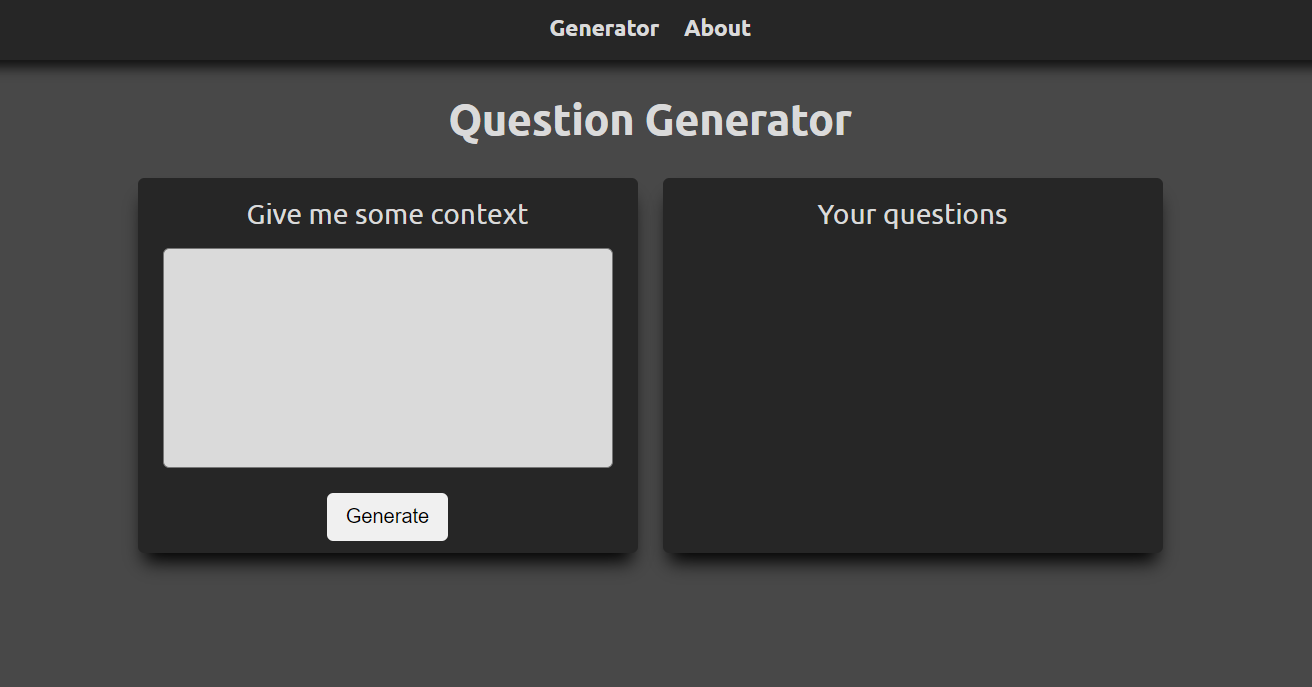
\includegraphics[scale=0.5]{images/app_ui.png}
\caption{A program felhasználói felülete.}
\label{fig:app_ui}
\end{figure}

A program nagyon egyszerű felhasználói interfészt használ. Adott 2 oldal: a főoldal és egy az alkalmazás leírását tartalmazó oldal. A főoldalon található maga a kérdésgeneráló komponens. A komponens bal oldalán lehet megadni a szöveges kontextust, ami alapján a kérdések generálódnak, míg a jobb oldalon fognak megjelenni az elkészült kérdések, könnyen másolható formában.

\begin{figure}[h]
\centering
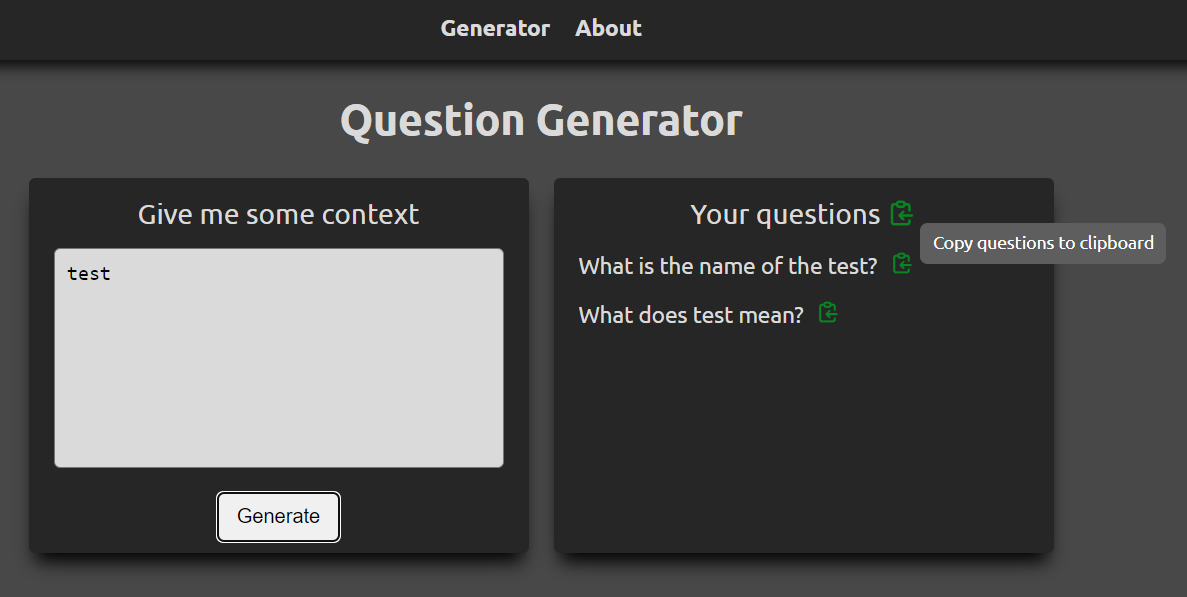
\includegraphics[scale=0.5]{images/app_ui_2.png}
\caption{Az elkészült kérdések.}
\label{fig:app_ui_2}
\end{figure}

\Section{Felhasznált programkönyvtárak bemutatása}

Mielőtt bemutatnám az alkalmazás részletes működését, szeretném ismertetni a felhasznált szerveroldali programkönyvtárakat(API-kat), melyek jelentősen megkönnyítették a fejlesztést.

\Section{A program részletes működése}
\Chapter{Tesztelés}

Ebben a fejezetben kerülnek bemutatásra az alkalmazáshoz készült automatikus, illetve manuális tesztek.

\Section{Automatikus tesztek}

Modern webalkalmazás lévén esetünkben is elengedhetetlen az automatikus tesztelés. Minden egyes funkcióhoz készültek egységtesztek, melyek biztosítják a megfelelő működésüket.

Szerveroldalon egyetlen fontos végpont van, amit tesztelni kellett, az pedig a \\
\textit{/api/generate-questions} útvonal.

\begin{figure}[h]
\centering
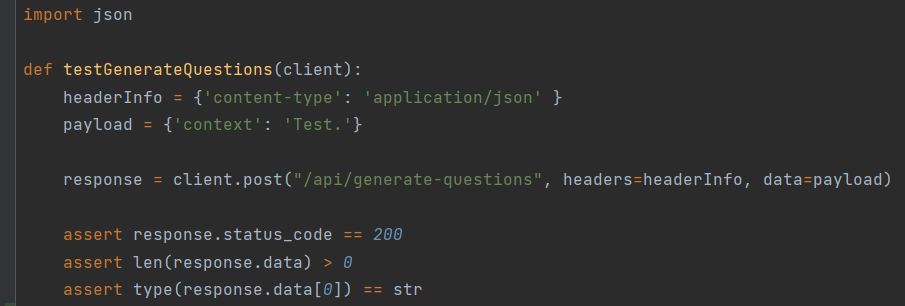
\includegraphics[scale=0.6]{images/test_backend_1.png}
\caption{A szerveroldali végpont egységtesztje.}
\label{fig:tb1}
\end{figure}

A \textbf{qg\_app\_backend} konténerbe terminállal belépve a \textit{pytest} parancs futtatásával lehet elindítani a szerveroldali teszteket. Ekkor minden \textbf{test} szót tartalmazó fájlt tesztnek érzékel és lefuttat a tesztkörnyezet.

\begin{figure}[h]
\centering
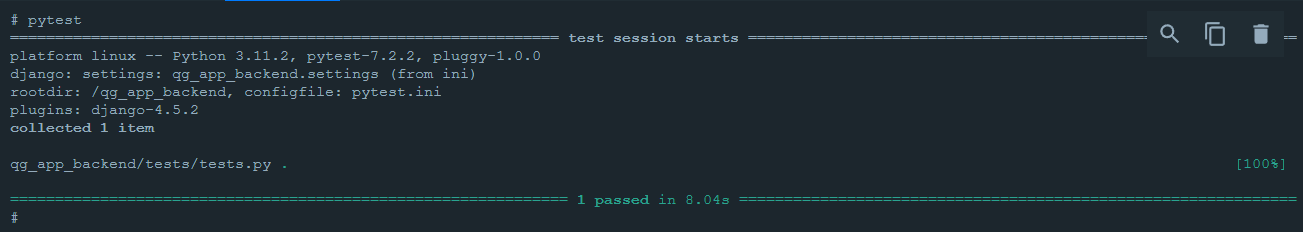
\includegraphics[scale=0.5]{images/test_backend_2.png}
\caption{A szerveroldali tesztek eredménye.}
\label{fig:tb2}
\end{figure}

\pagebreak

Kliens oldalon minden komponenshez készült egységteszt, melyek az adott komponenssel egy mappába kerültek elhelyezésre. Készült továbbá néhány integrációs teszt is az egyes oldalakhoz, illetve az alkalmazás egészéhez.

\begin{figure}[h]
\centering
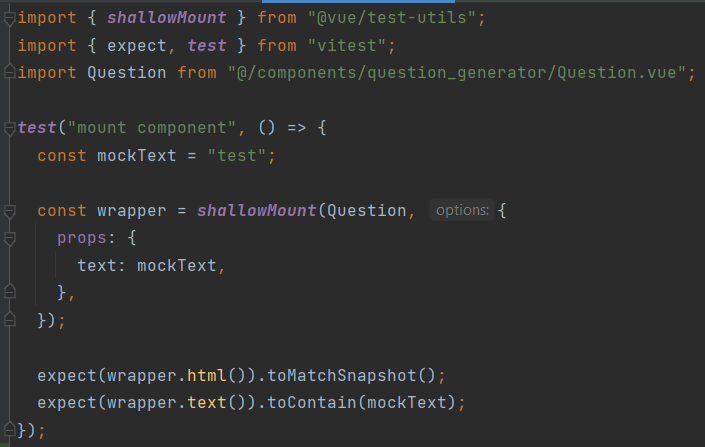
\includegraphics[scale=0.6]{images/test_frontend_1.png}
\caption{Question nevű komponens egységtesztje.}
\label{fig:tf1}
\end{figure}

\begin{figure}[h]
\centering
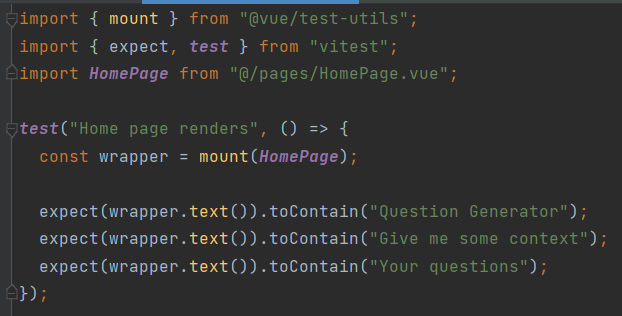
\includegraphics[scale=0.6]{images/test_frontend_2.png}
\caption{A főoldal integrációs tesztje.}
\label{fig:tf2}
\end{figure}

A kliensoldai egységtesztek futtatásához a \textbf{qg\_app\_frontend} konténerbe kell belépnünk és el kell indítanunk a \textit{npm run test} parancsot. Ekkor szintén minden kliensoldali \textbf{test} szót tartalmazó fájlban lefutnak a tesztek.

\pagebreak

\begin{figure}[h]
\centering
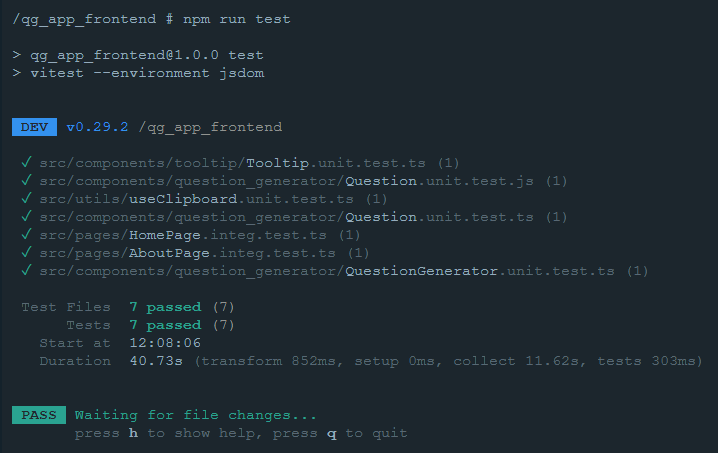
\includegraphics[scale=0.6]{images/test_frontend_3.png}
\caption{A kliensoldali tesztek eredménye.}
\label{fig:tf3}
\end{figure}

\Section{Manuális tesztek}

Mivel alkalmazásunk egy NLP feladat megoldására íródott, így elengedhetetlen, hogy kézzel is teszteljük. Ez esetünkben annyit jelentett, hogy különböző kontextusokat adtunk meg az alkalmazásnak és figyeltük, hogy milyen kérdéseket generált. Egy kérdés akkor számít elfogadottnak, ha értelmes, van köze a kontextushoz és nyelvtanilag is helyes.

\begin{figure}[h]
\centering
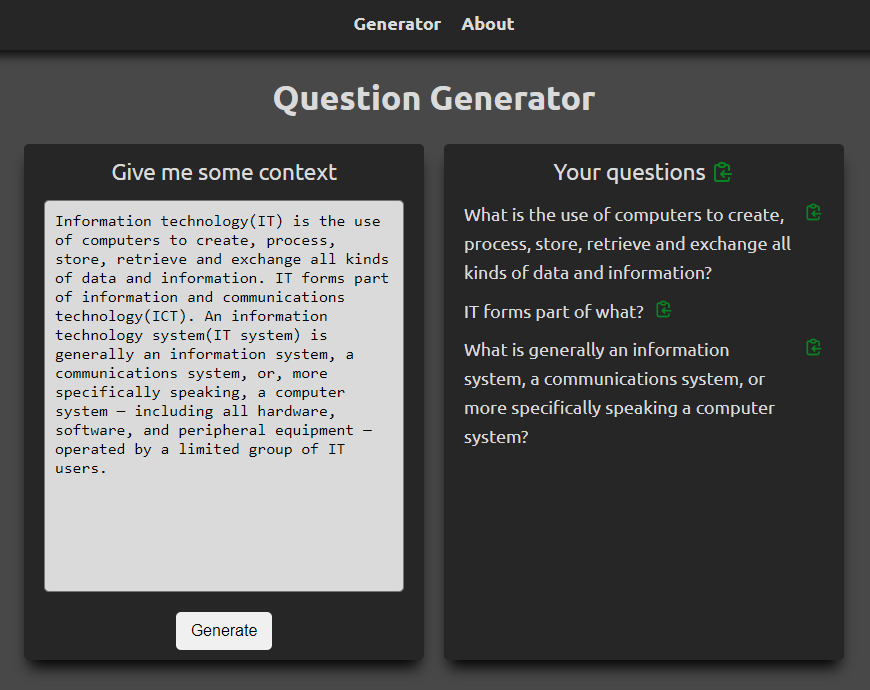
\includegraphics[scale=0.5]{images/test_manual.png}
\caption{Az alkalmazás egy manuális tesztje.}
\label{fig:tm}
\end{figure}

\pagebreak

A kezdeti tesztek elsősorban az alap működés ellenőrzésére szolgáltak, vagyis hogy képes-e az alkalmazás szavakból, mondatokból vagy hosszabb szövegekből kérdéseket generálni.

\begin{itemize}
\item \textbf{Kontextus:} "one"
\item \textbf{Kérdések:} 
	\begin{itemize}
		\item How many questions does one have to answer in order to get a good answer?
	\end{itemize}
	
\hrule	
	
\item \textbf{Kontextus:} "hungarian"
\item \textbf{Kérdések: }
	\begin{itemize}
		\item What is the nationality of the hungarian population?
		\item What country is the capital of Hungary?
	\end{itemize}
	
\hrule	
	
\item \textbf{Kontextus:} "Hungary is a country."
\item \textbf{Kérdések:}
	\begin{itemize}
		\item What is Hungary?
		\item What is a country?
	\end{itemize}
	
\hrule	
	
\item \textbf{Kontextus:} "Kate made an apple pie."
\item \textbf{Kérdések:}
	\begin{itemize}
		\item Kate made what kind of pie?
	\end{itemize}

\hrule	
	
\item \textbf{Kontextus:} "Information technology(IT) is the use of computers to create, process, store, retrieve and exchange all kinds of data and information. IT forms part of information and communications technology(ICT). An information technology system(IT system) is generally an information system, a communications system, or, more specifically speaking, a computer system — including all hardware, software, and peripheral equipment — operated by a limited group of IT users."
\item \textbf{Kérdések:}
	\begin{itemize}
		\item What is the use of computers to create, process, store, retrieve and exchange all kinds of data and information?
		\item IT forms part of what?
		\item What is generally an information system, a communications system, or more specifically speaking a computer system?
	\end{itemize}

\hrule

\item \textbf{Kontextus:} "A transformer is a deep learning model that adopts the mechanism of self-attention, differentially weighting the significance of each part of the input data. It is used primarily in the fields of natural language processing (NLP) and computer vision (CV). Like recurrent neural networks (RNNs), transformers are designed to process sequential input data, such as natural language, with applications towards tasks such as translation and text summarization. However, unlike RNNs, transformers process the entire input all at once. The attention mechanism provides context for any position in the input sequence. For example, if the input data is a natural language sentence, the transformer does not have to process one word at a time. This allows for more parallelization than RNNs and therefore reduces training times."
\item \textbf{Kérdések:}
	\begin{itemize}
		\item What is a deep learning model that adopts the mechanism of self-attention?
		\item What is used primarily in the fields of natural language processing (NLP) and computer vision (CV)?
		\item Like recurrent neural networks, transformers are designed to process what input data?
	\end{itemize}
\end{itemize}

Ezt követően elkezdtünk az alkalmazásnak különböző témakörökből kontextusokat megadni, hiszen célunk, hogy minél színesebb témaválasztékból tudjon a program kérdéseket generálni.

\begin{itemize}
\item \textbf{Témakör:} Fizika
\item \textbf{Kontextus:} "The Schrödinger equation is a linear partial differential equation that governs the wave function of a quantum-mechanical system. It is a key result in quantum mechanics, and its discovery was a significant landmark in the development of the subject. The equation is named after Erwin Schrödinger, who postulated the equation in 1925, and published it in 1926, forming the basis for the work that resulted in his Nobel Prize in Physics in 1933.
Conceptually, the Schrödinger equation is the quantum counterpart of Newton's second law in classical mechanics. Given a set of known initial conditions, Newton's second law makes a mathematical prediction as to what path a given physical system will take over time. The Schrödinger equation gives the evolution over time of a wave function, the quantum-mechanical characterization of an isolated physical system. The equation can be derived from the fact that the time-evolution operator must be unitary, and must therefore be generated by the exponential of a self-adjoint operator, which is the quantum Hamiltonian.
The Schrödinger equation is not the only way to study quantum mechanical systems and make predictions. The other formulations of quantum mechanics include matrix mechanics, introduced by Werner Heisenberg, and the path integral formulation, developed chiefly by Richard Feynman. Paul Dirac incorporated matrix mechanics and the Schrödinger equation into a single formulation. When these approaches are compared, the use of the Schrödinger equation is sometimes called "wave mechanics"."
\item \textbf{Kérdések:} 
	\begin{itemize}
		\item What is a linear partial differential equation that governs the wave function of a quantum-mechanical system?
		\item Who is the Schrödinger equation named after?
		\item What is the quantum counterpart of Newton's second law in classical mechanics?
		\item Which formulation of quantum mechanics was developed by Richard Feynman?
	\end{itemize}
	
\hrule	
	
\item \textbf{Témakör:} Történelem
\item \textbf{Kontextus:} "Hungary in its modern (post-1946) borders roughly corresponds to the Great Hungarian Plain (the Pannonian Basin). During the Iron Age, it was located at the crossroads between the cultural spheres of the Celtic tribes (such as the Scordisci, Boii and Veneti), Dalmatian tribes (such as the Dalmatae, Histri and Liburni) and the Germanic tribes (such as the Lugii and Marcomanni). The name "Pannonian" comes from Pannonia, a province of the Roman Empire. Only the western part of the territory (the so-called Transdanubia) of modern Hungary formed part of Pannonia. The Roman control collapsed with the Hunnic invasions of 370–410, and Pannonia was part of the Ostrogothic Kingdom during the late 5th to mid 6th century, succeeded by the Avar Khaganate (6th to 9th centuries). The Magyar invasion took place during the 9th century. The Magyars were Christianized at the end of the 10th century, and the Christian Kingdom of Hungary was established in 1000 under King Saint Stephen, ruled by the Árpád dynasty for the following three centuries. In the high medieval period, the kingdom expanded to the Adriatic coast and entered a personal union with Croatia during the reign of King Coloman in 1102. In 1241 during the reign of King Béla IV, Hungary was invaded by the Mongols under Batu Khan. The outnumbered Hungarians were decisively defeated at the Battle of Mohi by the Mongol army. In this invasion more than 500,000 Hungarian people were massacred and the whole kingdom reduced to ashes. The paternal lineage of the ruling Árpád dynasty came to end in 1301, and all of the subsequent kings of Hungary (with the exception of King Matthias Corvinus) were cognatic descendants of the Árpád dynasty. Hungary bore the brunt of the Ottoman wars in Europe during the 15th century. The peak of this struggle took place during the reign of Matthias Corvinus (r. 1458–1490). The Ottoman–Hungarian wars concluded in significant loss of territory and the partition of the kingdom after the Battle of Mohács of 1526."
\item \textbf{Kérdések:} 
	\begin{itemize}
		\item What is the Pannonian Basin?
		\item Who invaded Hungary in 1241?
		\item How many people were massacred in the Battle of Mohi?
		\item When did the Ottoman-Hungarian wars end?
	\end{itemize}
	
\hrule	
	
\item \textbf{Témakör:} Biológia
\item \textbf{Kontextus:} "A virus is a submicroscopic infectious agent that replicates only inside the living cells of an organism. Viruses infect all life forms, from animals and plants to microorganisms, including bacteria and archaea. Since Dmitri Ivanovsky's 1892 article describing a non-bacterial pathogen infecting tobacco plants and the discovery of the tobacco mosaic virus by Martinus Beijerinck in 1898, more than 9,000 of the millions of virus species have been described in detail. Viruses are found in almost every ecosystem on Earth and are the most numerous type of biological entity. The study of viruses is known as virology, a subspeciality of microbiology. When infected, a host cell is often forced to rapidly produce thousands of copies of the original virus. When not inside an infected cell or in the process of infecting a cell, viruses exist in the form of independent viral particles, or virions, consisting of the genetic material, i.e., long molecules of DNA or RNA that encode the structure of the proteins by which the virus acts; a protein coat, the capsid, which surrounds and protects the genetic material; and in some cases  an outside envelope of lipids. The shapes of these virus particles range from simple helical and icosahedral forms to more complex structures. Most virus species have virions too small to be seen with an optical microscope and are one-hundredth the size of most bacteria. The origins of viruses in the evolutionary history of life are unclear: some may have evolved from plasmids—pieces of DNA that can move between cells—while others may have evolved from bacteria. In evolution, viruses are an important means of horizontal gene transfer, which increases genetic diversity in a way analogous to sexual reproduction. Viruses are considered by some biologists to be a life form, because they carry genetic material, reproduce, and evolve through natural selection, although they lack the key characteristics, such as cell structure, that are generally considered necessary criteria for defining life. Because they possess some but not all such qualities, viruses have been described as "organisms at the edge of life" and as replicators."
\item \textbf{Kérdések:} 
	\begin{itemize}
		\item What is a submicroscopic infectious agent that replicates only inside the living cells of an organism?
		\item How many of the millions of virus species have been described in detail since Dmitri Ivanovsky's 1892 article?
		\item What is the study of viruses known as?
	\end{itemize}

\hrule

\item \textbf{Témakör:} Informatika
\item \textbf{Kontextus:} "In computing, a server is a piece of computer hardware or software (computer program) that provides functionality for other programs or devices, called "clients." This architecture is called the client–server model. Servers can provide various functionalities, often called "services," such as sharing data or resources among multiple clients or performing computations for a client. A single server can serve multiple clients, and a single client can use multiple servers. A client process may run on the same device or may connect over a network to a server on a different device. Typical servers are database servers, file servers, mail servers, print servers, web servers, game servers, and application servers. Client–server systems are usually most frequently implemented by (and often identified with) the request–response model: a client sends a request to the server, which performs some action and sends a response back to the client, typically with a result or acknowledgment. Designating a computer as "server-class hardware" implies that it is specialized for running servers on it. This often implies that it is more powerful and reliable than standard personal computers, but alternatively, large computing clusters may be composed of many relatively simple, replaceable server components."
\item \textbf{Kérdések:} 
	\begin{itemize}
		\item What is a piece of computer hardware or software that provides functionality for other programs or devices called?
		\item What architecture is called the client-server model?
		\item Servers can provide various functionalities, often called what?
		\item A single server can serve multiple clients, and a single client can use multiple servers?
	\end{itemize}

\hrule

\item \textbf{Témakör:} Földrajz
\item \textbf{Kontextus:} "Earth is the third planet from the Sun and the only place known in the universe where life has originated and found habitability. While Earth may not contain the largest volumes of water in the Solar System, only Earth sustains liquid surface water, extending over 70.8\% of the Earth with its ocean, making Earth an ocean world. Earth's polar regions currently retain most of all other water with large sheets of ice covering ocean and land, dwarfing Earth's groundwater, lakes, rivers and atmospheric water. Land, consisting of continents and islands, extends over 29.2\% of the Earth and is widely covered by vegetation. Below Earth's surface material lies Earth's crust consisting of several slowly moving tectonic plates, which interact to produce mountain ranges, volcanoes, and earthquakes. Earth's liquid outer core generates a magnetic field that shapes the magnetosphere of Earth, largely deflecting destructive solar winds and cosmic radiation."
\item \textbf{Kérdések:} 
	\begin{itemize}
		\item What planet is the third from the Sun?
		\item What is the only place known in the universe where life has originated and found habitability?
		\item Earth's liquid outer core generates a magnetic field that shapes the magnetosphere of what?
	\end{itemize}
\end{itemize}

\Section{Összehasonlítás a ChatGPT-vel}

Mivel mostanság nagyon elterjedtek a különböző általános NLP feladatokat megoldó szöveggenerátorok, így elengedhetetlen volt, hogy alkalmazásunkat összehasonlítsuk egy másik, hasonló programmal. A ChatGPT-re esett a választás, mivel jelenleg ez az egyik legnépszerűbb és legjobb teljesítményt elért program a piacon.
\begin{itemize}
\item \textbf{Kontextus:} "Thomas ate an apple."
\item \textbf{Alkalmazásunk kérdései:} 
	\begin{itemize}
		\item What did Thomas eat?
	\end{itemize}
\item \textbf{ChatGPT kérdései:} 
	\begin{itemize}
		\item What did Thomas eat?
	\end{itemize}

\hrule

\item \textbf{Kontextus:} "Claire went to the store and bought some vegetables, fish, butter and shampoo."
\item \textbf{Alkalmazásunk kérdései:} 
	\begin{itemize}
		\item Claire went to the store and bought what?
		\item What did Claire buy at the store?
	\end{itemize}
\item \textbf{ChatGPT kérdései:} 
	\begin{itemize}
		\item What items did Claire purchase when she went to the store?
	\end{itemize}
	
\hrule	
	
\item \textbf{Kontextus:} "One day, a fox became very hungry as he went to search for some food. He searched high and low, but couldn’t find something that he could eat.
Finally, as his stomach rumbled, he stumbled upon a farmer’s wall. At the top of the wall, he saw the biggest, juiciest grapes he’d ever seen. They had a rich, purple color, telling the fox they were ready to be eaten. To reach the grapes, the fox had to jump high in the air. As he jumped, he opened his mouth to catch the grapes, but he missed. The fox tried again but missed yet again. He tried a few more times but kept failing. Finally, the fox decided it was time to give up and go home. While he walked away, he muttered, “I’m sure the grapes were sour anyway.”"
\item \textbf{Alkalmazásunk kérdései:} 
	\begin{itemize}
		\item What did a fox do when he became hungry?
		\item What color did the grapes on the wall tell the fox they were ready to be eaten?
		\item The fox had to jump high in the air to reach what?
	\end{itemize}
\item \textbf{ChatGPT kérdései:}
	\begin{itemize}
		\item What did the fox do when he became very hungry?
		\item Where did the fox search for food?
		\item What did the fox find when he stumbled upon a farmer’s wall?
		\item How did the fox feel when he saw the grapes?
		\item What did the fox have to do to reach the grapes?
	\end{itemize}
	
\hrule	
	
\item \textbf{Kontextus:} "The London Zoo, which was opened in 1828, was initially known as the "Gardens and Menagerie of the Zoological Society of London", and it described itself as a menagerie or "zoological forest". The abbreviation "zoo" first appeared in print in the United Kingdom around 1847, when it was used for the Clifton Zoo, but it was not until some 20 years later that the shortened form became popular in the rhyming song "Walking in the Zoo" by music-hall artist Alfred Vance. The term "zoological park" was used for more expansive facilities in Halifax, Nova Scotia, Washington, D.C., and the Bronx in New York, which opened in 1847, 1891 and 1899 respectively. Relatively new terms for zoos in the late 20th century are "conservation park" or "bio park". Adopting a new name is a strategy used by some zoo professionals to distance their institutions from the stereotypical and nowadays criticized zoo concept of the 19th century. The term "bio park" was first coined and developed by the National Zoo in Washington D.C. in the late 1980s. In 1993, the New York Zoological Society changed its name to the Wildlife Conservation Society and re branded the zoos under its jurisdiction as "wildlife conservation parks"."
\item \textbf{Alkalmazásunk kérdései:} 
	\begin{itemize}
		\item When was the London Zoo opened?
		\item When did the abbreviation "zoo" first appear in print in the United Kingdom?
		\item What did Alfred Vance's song "Walking in the Zoo" become popular in?
		\item In what year did the New York Zoological Society change its name to?
	\end{itemize}
\item \textbf{ChatGPT kérdései:} 
	\begin{itemize}
		\item When was the London Zoo opened and what was its original name?
		\item How did the abbreviation "zoo" come into use in the United Kingdom?
		\item Who popularized the term "zoo" in a rhyming song and when was it released?
		\item What are some examples of facilities that were referred to as "zoological parks" in the 19th century?
		\item What are some of the relatively new terms used for zoos in the late 20th century?
		\item Why do some zoo professionals adopt new names for their institutions?
		\item Which zoo first coined the term "bio park" and when was it developed?
		\item In what year did the New York Zoological Society change its name and rebrand its zoos as "wildlife conservation parks"?
	\end{itemize}
	
\hrule	
	
\item \textbf{Kontextus:} "In computing, a database is an organized collection of data stored and accessed electronically. Small databases can be stored on a file system, while large databases are hosted on computer clusters or cloud storage. The design of databases spans formal techniques and practical considerations, including data modeling, efficient data representation and storage, query languages, security and privacy of sensitive data, and distributed computing issues, including supporting concurrent access and fault tolerance. A database management system (DBMS) is the software that interacts with end users, applications, and the database itself to capture and analyze the data. The DBMS software additionally encompasses the core facilities provided to administer the database. The sum total of the database, the DBMS and the associated applications can be referred to as a database system. Often the term "database" is also used loosely to refer to any of the DBMS, the database system or an application associated with the database. Computer scientists may classify database management systems according to the database models that they support. Relational databases became dominant in the 1980s. These model data as rows and columns in a series of tables, and the vast majority use SQL for writing and querying data. In the 2000s, non-relational databases became popular, collectively referred to as NoSQL, because they use different query languages."
\item \textbf{Alkalmazásunk kérdései:} 
	\begin{itemize}
		\item What is an organized collection of data stored and accessed electronically?
		\item Where are large databases hosted?
		\item What is the software that interacts with end users, applications, and the database itself to capture and analyze the data?
		\item When did relational databases become dominant?
	\end{itemize}
\item \textbf{ChatGPT kérdései:} 
	\begin{itemize}
		\item What is a database in computing?
		\item How are small databases stored compared to large databases?
		\item What are some practical considerations in the design of databases?
		\item What is a database management system (DBMS)?
		\item What is the role of DBMS software in capturing and analyzing data?
	\end{itemize}
\end{itemize}
\Chapter{Összegzés}

Mint láthattuk dolgozatomban is, a természetes nyelvfeldolgozás virágkorát éli napjainkban. Egymás után jelennek meg olyan alkalmazások, chatbotok melyek szinte tökéletesen képesek megérteni az emberi nyelveket, képesek szöveges feladatokat megoldani, kódokat generálni, cikkeket értelmezni és írni, szöveges hibákat keresni vagy ahogy láthattuk is immáron képesek értelmes kérdéseket is generálni nagyon jó eredményekkel. 

Úgy gondolom, hogy alkalmazásunk remekül beilleszthető ezen megoldások mellé, de nyilván van rajta még javítani való. Láthattuk, hogy a ChatGPT-vel összehasonlítva azért teljesítményben van még hova fejlődnie, de kisebb mérete és jobb hardvereken való gyorsabb teljesítménye, így is számos plusz pontot ad programunknak.

Ahol lehetne még fejleszteni az alkalmazást az mindenképp a tudásbázisa. Amellett, hogy többnyelvűvé is lehetne tenni, növelni lehetne a tudását egy jobban szűrt, többféle kérdés és kontextustípust is tartalmazó tanítóhalmazzal. Továbbá nem ártana a hardveres erőforrásokon is javítani és egy még nagyobb, GPU-t vagy TPU-t kihasználó felhőszolgáltatáson taníttatni és működtetni, ahol kihozhatnánk belőle a maximumot. Ez természetesen a többi neurális hálózatokat használó alkalmazás problémája is, hiszen a hálózat méretét növelve egyre jelentősebb lesz a teljesítményigény is, így többnyire nagyobb cégek tudnak ezekhez megfelelő erőforrásokat biztosítani.

Ehhez kapcsolódóan fontos kérdés lehet még ezen mély tanulás alapú megoldások, illetve magának az informatikai szektornak a teljesítményigénye, hiszen egy-egy komolyabb modell tanítása óriási költségekkel járhat, ami a hibajavítást is megnehezítheti, hiszen nagyobb volumenű hibáknál sokszor nincs lehetőség az egész hálózatot újratanítani, mivel az akár hónapokig is eltarthat és rengeteg erőforrást felemészthet. Természetesen a technológia fejlődése itt is megoldhatja a problémákat, de a jövőben erre mindenképp oda kell majd figyelni.

Végül fontosnak tartom még megemlíteni az ilyen neurális hálózat alapú, NLP megoldások társadalmunkat is érintő következményeit. Világosan látszik, hogy közelítünk egy olyan ponthoz, ahol a 20. században felvázolt gépi intelligenciát behatároló korlátokat kezdjük átlépni. Sorra jelennek meg olyan alkalmazások a terület kutatásai alapján, melyek képesek megoldani olyan feladatokat, amiket eddig csak emberek, külön képesítéssel tudtak elvégezni, azonban egyre többször találkozhatunk azzal is, hogy a gép szintaktikailag jól oldotta meg a feladatot, de valójában helytelen eredményeket generált. Úgy gondolom ezen a területen is rengeteget kell még fejlődnie a tudománynak és a neurális hálózatokat önmagyarázóvá és könnyebben karbantarthatóvá kell tenni, más különben eláraszthatják az internetet hamis, pontatlan információkkal, amik egy láncreakció folytán a később modellek eredményeit is ronthatják, illetve társadalmunkra is negatív hatással lehetnek.

Úgy vélem dolgozatom jó táptalaj lehet ezen megoldások elkészítéséhez a jövőben és én is törekedni fogok a terület népszerűsítésére és kutatására az elkövetkezendőkben.

\Chapter{Summary}

As we saw in my thesis, natural language processing is currently in its heyday. Applications and chatbots appear one after another that are able to understand human languages almost perfectly, are able to solve text tasks, generate codes, interpret and write articles, search for text errors or, as we have seen, are now able to generate meaningful questions with very good results.

I think that our application can be perfectly integrated with these solutions, but there is obviously room for improvement. We could see that, compared to ChatGPT, it still has room for improvement in terms of performance, but its smaller size and faster performance on better hardware still give our program many plus points.

Where the application could still be improved is definitely its knowledge base. In addition to making it multilingual, it's knowledge could be increased with a more filtered training set containing several types of questions and contexts. Furthermore, it would not hurt to improve the hardware resources and have it taught and operated on an even larger cloud service that uses GPU or TPU, where we could get the most out of it. This is, of course, also the problem of other applications using neural networks, since increasing the size of the network will also increase the performance requirements, so mostly larger companies can provide adequate resources for these.

Relatedly, these deep learning-based solutions and the performance requirements of the IT sector itself can also be an important issue, since training a serious model can entail enormous costs, which can also make error correction difficult, since it is often not possible to retrain the entire network in the case of large-volume errors, since it can take months and consume a lot of resources. Of course, the development of technology can solve the problems here as well, but in the future we will definitely have to pay attention to this.

Finally, I consider it important to mention the consequences of such neural network-based NLP solutions that also affect our society. It is clear that we are approaching a point where we are starting to cross the boundaries of machine intelligence outlined in the 20th century. Applications based on research in the field are appearing one after another, which are able to solve tasks that until now only humans, with special qualifications, could do, but we can also come across more and more that the machine solved the task syntactically well, but actually generated incorrect results. I think that science still needs to improve a lot in this area and neural networks need to be made self-explanatory and easier to maintain, otherwise they can flood the internet with false and inaccurate information, which, due to a chain reaction, can worsen the results of later models and have a negative impact on our society. .

I believe that my thesis can be a good breeding ground for preparing these solutions in the future, and I will also strive to popularize and research the field in the future.

\addcontentsline{toc}{chapter}{Irodalomjegyzék}
\bibliographystyle{unsrt}
\begin{thebibliography}{100}
\bibitem{rnn} Recurrent neural network unfold, \url{https://commons.wikimedia.org/wiki/File:Recurrent\_neural\_network\_unfold.svg}

\bibitem{attention} Vaswani, Ashish and Shazeer, Noam and Parmar, Niki and Uszkoreit, Jakob and Jones, Llion and Gomez, Aidan and Kaiser, Lukasz and Polosukhin, Illia. (2017). Attention Is All You Need.

\bibitem{translation} Bahdanau, Dzmitry and Cho, Kyunghyun and Bengio, Y.. (2014). Neural Machine Translation by Jointly Learning to Align and Translate. ArXiv. 1409.

\bibitem{bert} Tassopoulou, Vasiliki. (2019). An Exploration of Deep Learning Architectures for Handwritten Text Recognition. 10.13140/RG.2.2.34041.62565.

\bibitem{bert2} Devlin, Jacob and Chang, Ming-Wei and Lee, Kenton and Toutanova, Kristina. (2018). BERT: Pre-training of Deep Bidirectional Transformers for Language Understanding.

\bibitem{t5} Exploring Transfer Learning with T5: the Text-To-Text Transfer Transformer https://ai.googleblog.com/2020/02/exploring-transfer-learning-with-t5.html
\end{thebibliography}


\noindent \textit{Az internetes források utolsó ellenőrzése: 2022.08.23}

\pagestyle{empty}

\newpage

\pagestyle{empty}

\noindent \textbf{\Large CD melléklet tartalma}

\vskip 1cm

\noindent A dolgozathoz mellékelt lemezen egy \texttt{Dolgozat} nevű jegyzékben a következő fájlok találhatóak.

\begin{itemize}
\item A dolgozat \LaTeX\ forráskódja.
\item A dolgozat PDF formátumban (\texttt{dolgozat.pdf}).
\item A magyar és angol nyelvű összefoglaló \LaTeX\ és PDF formátumban \\ (\texttt{osszegzes.tex}, \texttt{osszegzes.pdf}, \texttt{summary.tex}, \texttt{summary.pdf}).
\end{itemize}

A \texttt{Program} nevű jegyzékben található a dolgozathoz elkészített program forráskódja és futtatható változata.

\begin{itemize}
\item \textit{Feladattól, technológiától függően ez változhat.}
\item \textit{Konkretizálni kell, hogy pontosan mit tartalmaz a jegyzék!}
\end{itemize}


\end{document}
